% q4_models.tex - Question 4 parts 3(c) 3(d) 3(e) (OWNER: E) - prose integrated verbatim from report/Q4_E_report_final.md
\subsection*{4.3(c) Model specification and selection}

The response log(streams) is continuous and approximately symmetric after the log transformation shown in Figure Q4-D2, so we fitted generalized linear models with the Gaussian family and identity link using \texttt{glm()}; this is equivalent to ordinary linear regression on the log scale. Following the research question, we compared three nested candidate models:

\begin{itemize}
  \item m1: $\log(\text{streams}) \sim \log(\text{in\_QQ\_playlists})$
  \item m2: $\log(\text{streams}) \sim \log(\text{in\_QQ\_playlists}) + \text{artist\_count} + \text{released\_year}$
  \item m3: $\log(\text{streams}) \sim \log(\text{in\_QQ\_playlists}) + \text{artist\_count} + \text{released\_year} + \text{danceability\_\%} + \text{energy\_\%} + \text{acousticness\_\%}$
\end{itemize}

Adding artist count and release year improves fit significantly (nested F test: $F = 9.288$, $\pval < 0.001$), whereas adding the three audio features does not ($F = 0.842$, $\pval = 0.471$). The AIC agrees: 1876.172, 1861.700 and 1865.156 for m1, m2 and m3 respectively (Table Q4-E1), so m2 is preferred by both criteria. The final model is therefore

\[
\log(\text{streams}) = 3.157 + 0.689 \cdot \log(\text{in\_QQ\_playlists}) - 0.114 \cdot \text{artist\_count} + 0.006 \cdot \text{released\_year},
\]

fitted on $n = 843$ songs with residual deviance 443.92 on 839 degrees of freedom ($R^2 = 0.614$). Variance inflation factors for the final model are at most 1.192 (Table Q4-E4), consistent with D's candidate-set check of 1.058 to 1.627, so multicollinearity is not a concern.

\begin{table}[htbp]
  \centering
  \caption*{Table Q4-E1: Model comparison by AIC.}
  \begin{tabular}{llr}
    \toprule
    Model & Specification & AIC \\
    \midrule
    m1 & log\_playlists & 1876.172 \\
    m2 & + artist\_count + released\_year & 1861.700 \\
    m3 & + danceability + energy + acousticness & 1865.156 \\
    \bottomrule
  \end{tabular}
\end{table}

Two coefficients in context. First, the elasticity of playlist inclusion is 0.689 (95\% CI $[0.649,\ 0.729]$, $t = 33.790$, $\pval < 0.001$): each 1\% increase in the number of QQ Music playlists including a song is associated with an approximately 0.689\% higher geometric-mean stream count, holding artist count and release year fixed; doubling playlist inclusions corresponds to a multiplicative factor of $2^{0.689} \approx 1.616$, i.e.\ about 61.6\% higher streams. Second, each additional contributing artist is associated with a multiplicative factor of $e^{-0.114} \approx 0.892$ (95\% CI for the coefficient $[-0.173,\ -0.055]$, $\pval < 0.001$), that is, about 10.8\% lower streams for collaborations of a given playlist exposure and release year. The release-year coefficient is small and positive (0.006, 95\% CI $[0.001,\ 0.010]$, $\pval = 0.025$); we interpret it cautiously because release year is an imperfect proxy for time available to accumulate streams. The elasticity estimate is essentially unchanged across m1, m2 and m3 (0.678, 0.689 and 0.692; Table Q4-E2), so the adjusted association between playlist inclusion and streams is robust to which controls enter the model.

\begin{table}[htbp]
  \centering
  \caption*{Table Q4-E2: Elasticity of log playlist inclusions across candidate models.}
  \begin{tabular}{lrr}
    \toprule
    Model & log\_playlists coefficient & $R^2$ \\
    \midrule
    m1 & 0.678 & 0.606 \\
    m2 & 0.689 & 0.614 \\
    m3 & 0.692 & 0.615 \\
    \bottomrule
  \end{tabular}
\end{table}

\begin{table}[htbp]
  \centering
  \small
  \caption*{Table Q4-E3: Final model (m2) coefficients with 95\% confidence intervals.}
  \begin{tabular}{lrrrrrr}
    \toprule
    Term & Estimate & SE & $t$ & $\pval$ & 2.5\% & 97.5\% \\
    \midrule
    (Intercept) & 3.157 & 5.051 & 0.625 & 0.532 & $-6.744$ & 13.057 \\
    log\_playlists & 0.689 & 0.020 & 33.790 & $< 0.001$ & 0.649 & 0.729 \\
    artist\_count & $-0.114$ & 0.030 & $-3.811$ & $< 0.001$ & $-0.173$ & $-0.055$ \\
    released\_year & 0.006 & 0.002 & 2.245 & 0.025 & 0.001 & 0.010 \\
    \bottomrule
  \end{tabular}
\end{table}

\begin{table}[htbp]
  \centering
  \caption*{Table Q4-E4: Variance inflation factors for the final model (m2).}
  \begin{tabular}{lr}
    \toprule
    Term & VIF \\
    \midrule
    log\_playlists & 1.192 \\
    artist\_count & 1.013 \\
    released\_year & 1.192 \\
    \bottomrule
  \end{tabular}
\end{table}

\subsection*{4.3(d) Diagnostics and prediction}

Figure Q4-E1 shows the four standard residual plots for the final model. Residuals against fitted values show no remaining systematic curvature, supporting the linearity of the log-log specification. The normal Q-Q plot is close to linear in the centre with somewhat heavier tails, which is common for large observational datasets; the residual-vs-log-playlists plot (Figure Q4-E2) shows no trend in location or spread across the observed range of playlist inclusions. The scale-location plot shows mildly increasing spread at high fitted values, indicating mild heteroscedasticity rather than a structural failure. The largest Cook's distance is 0.184 (``Dream On''), with all values far below levels that would indicate a single influential observation, so no records were removed.

\begin{figure}[htbp]
  \centering
  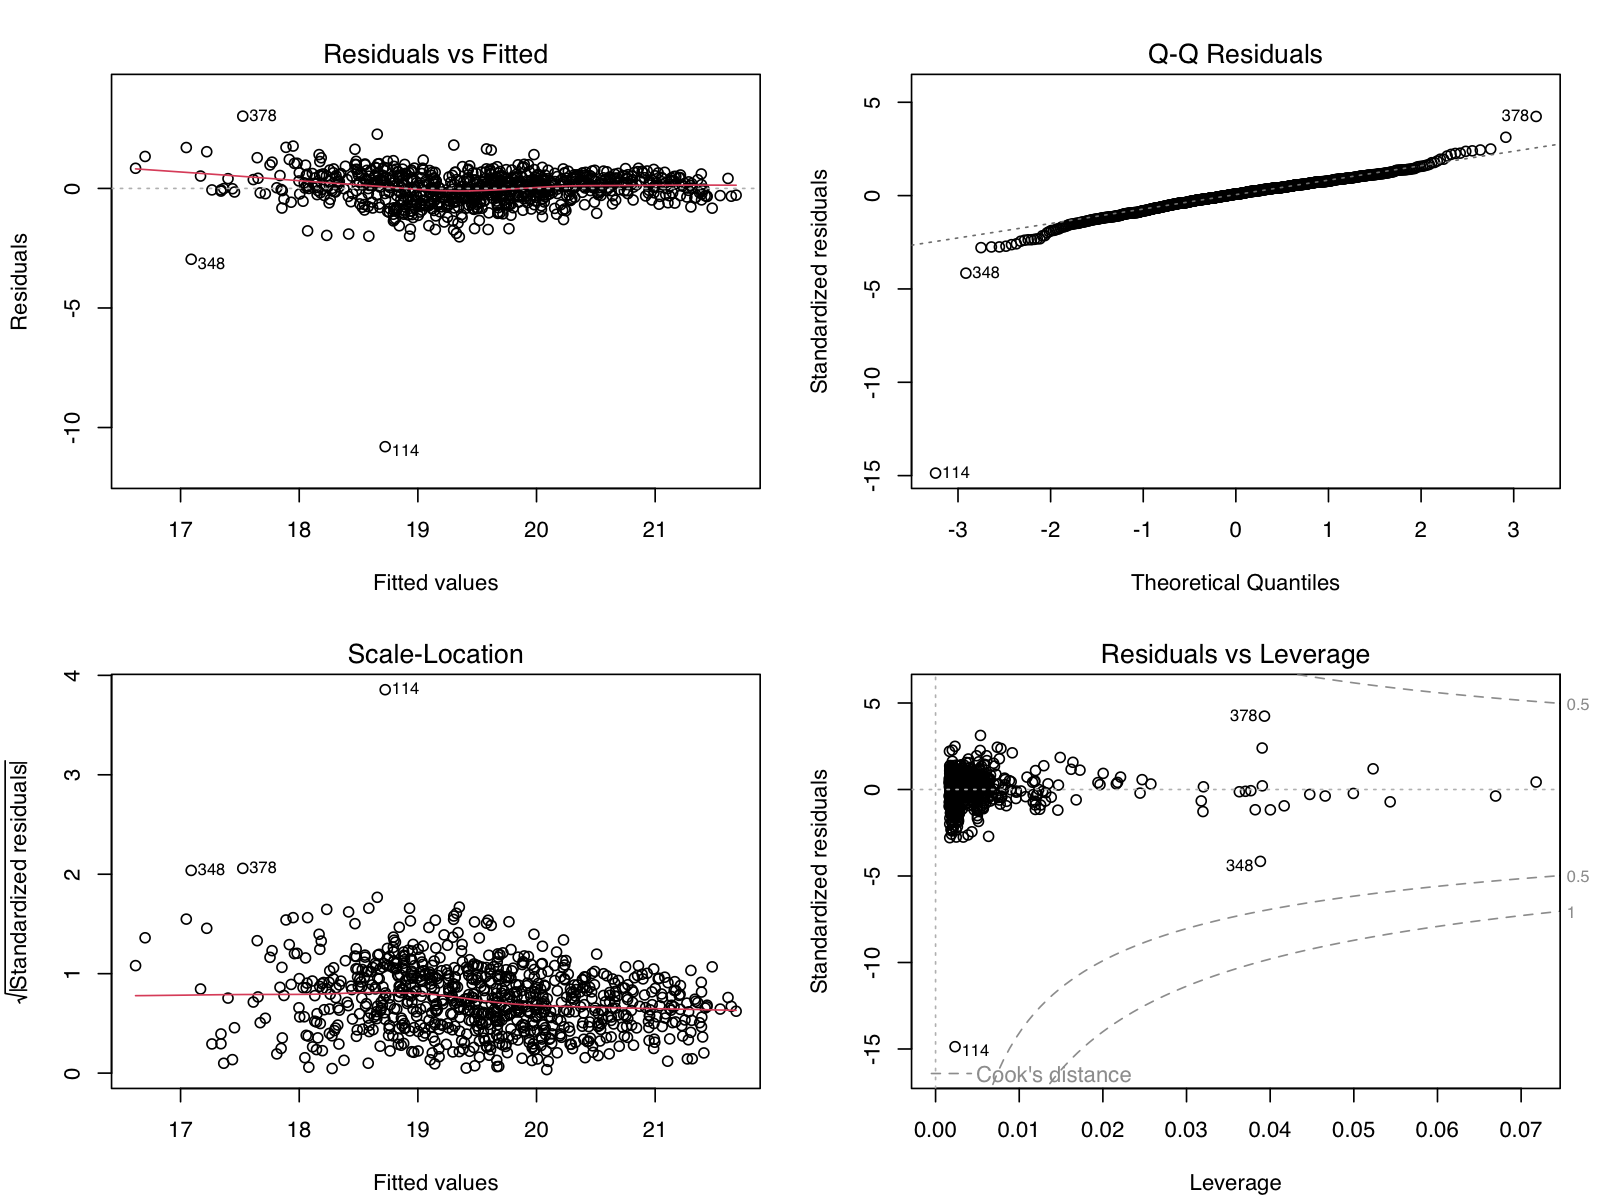
\includegraphics[width=0.9\textwidth]{Q4_E_Figure_01_diagnostics.png}
  \caption*{Figure Q4-E1: The four standard residual plots for the final model.}
\end{figure}

\begin{figure}[htbp]
  \centering
  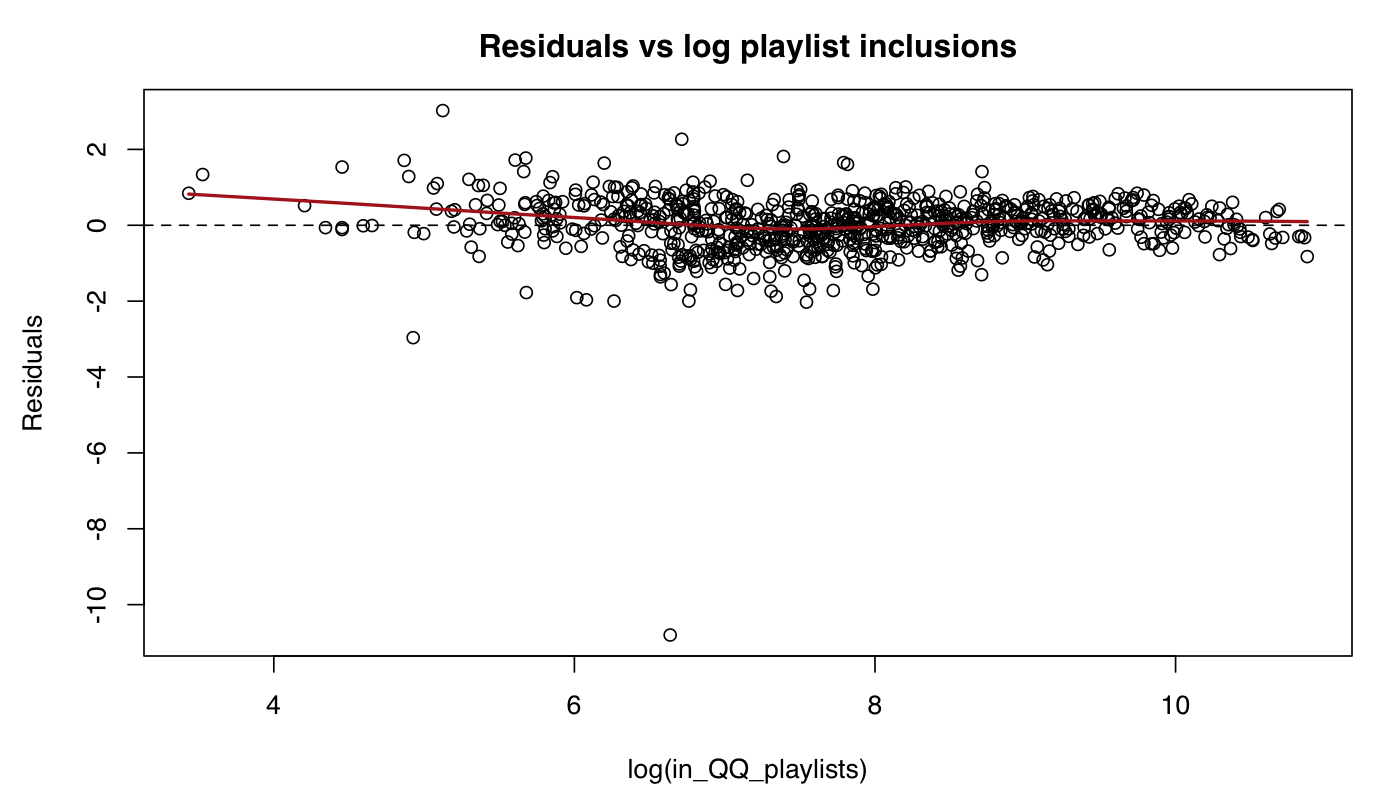
\includegraphics[width=0.85\textwidth]{Q4_E_Figure_02_residual_vs_log_playlists.png}
  \caption*{Figure Q4-E2: Residuals versus log playlist inclusions.}
\end{figure}

For prediction we defined a plausible scenario within the observed predictor ranges: a song included in the median number of playlists (2,313), with the median artist count (1) and median release year (2022). The predicted mean log streams is 19.606. The 95\% confidence interval for the mean response is $[306.753,\ 346.730]$ million streams: with 95\% confidence, the average log streams of songs with these characteristics lies in this range on the original scale. The 95\% prediction interval for a single new song with these characteristics is much wider, $[78.281,\ 1358.702]$ million streams, because it additionally accounts for song-to-song variability; the width of this interval reflects the large residual variation in individual streaming outcomes.

\begin{table}[htbp]
  \centering
  \small
  \caption*{Table Q4-E5: Prediction at the median scenario (playlists $= 2313$, artist count $= 1$, release year 2022).}
  \begin{tabular}{lll}
    \toprule
    Quantity & Interval, log scale & Interval, million streams \\
    \midrule
    Mean response CI & $[19.542,\ 19.664]$ & $[306.753,\ 346.730]$ \\
    New observation PI & $[18.176,\ 21.030]$ & $[78.281,\ 1358.702]$ \\
    \bottomrule
  \end{tabular}
\end{table}

\subsection*{4.3(e) Conclusion and model justification}

We answered the research question with a Gaussian GLM on log(streams), selecting the final model by nested F tests and AIC among three candidates that progressively added artist count and release year, then the three audio features. Both criteria preferred the model with playlist inclusion, artist count and release year (AIC $= 1861.700$); the audio features added no significant improvement ($\pval = 0.471$) and did not change the substantive conclusion.

The central finding is a strong, robust positive adjusted association between playlist inclusion and streams: the elasticity is 0.689 (95\% CI $[0.649,\ 0.729]$), stable at 0.678--0.692 across all candidate models, so songs included in more QQ Music playlists have substantially higher stream counts even after accounting for artist count, release year and audio characteristics. Collaborations are associated with about 10.8\% lower streams at equal playlist exposure. For the QQ Music team, this quantifies how strongly playlist reach tracks streaming performance and supports treating playlist placement as a key visibility lever, although reverse causality is plausible: popular songs are also more likely to be added to playlists.

Limitations: the data are observational, so coefficients describe associations rather than causal effects of playlist placement; unmeasured factors such as label promotion and artist fame may drive both inclusion and streams; release year imperfectly measures accumulation time; diagnostics indicate mildly heavy-tailed residuals and mild heteroscedasticity; and the wide prediction interval shows that individual song outcomes remain highly variable.
